\dev{Emile Martinez}{}

\section{Introduction}

\begin{definition}[Paradigme Diviser pour Régner]Un algorithme de type Diviser pour Régner s'effectue en 3 étapes : \begin{enumerate}
		\item Division du problème en sous-problèmes indépendants
		\item Résolution récursive des sous-problèmes
		\item Construction d'une solution du problème global à partir des solutions des sous-problèmes
\end{enumerate}
	
\end{definition}

\begin{principe}[Calcul de la compléxité d'un tel algorithme.]
	
	Trouver une fonction donnant la taille du problème (comme le nombre d'éléments pour une liste). Définir $C$ la complexité maximale des instances de cette taille, puis trouver une relation de réccurence sur $C$, pour tenter de la résoudre.
	
\end{principe}

\begin{com}
	La méthode de résolution sera inculqué par l'exemple, et progressivement (d'abord le cas de base, où l'on découpe en seulement 2 avec l'exponentiation rapide, puis on complexifie)
\end{com}

\section{Applications au calcul formel}

\subsection{L'exponentiation rapide}

\textbf{Problème :} Étant donné un entier $a$ et un entier positif $n$, calculer $a^n$.

\textbf{Solution naïve :} $n$ multiplications

\begin{algo}[Méthode D\&R] \enspace \\
	\begin{minipage}{0.7\linewidth}
		\begin{algorithm}[H]
			\caption{$exponentiation\_rapide(a, n)$}
			\Si{$n = 0$}
				{\Retour{$1$}}
			$m \gets m/2$ \tcp*{étape 1}
			$x \gets exponentiation\_rapide(a, m)$ \tcp*{étape 2}
			\eSi(\tcp*{étape 3}){$n$ est pair}
				{\Retour{$x\times x$}}
				{\Retour{$x\times x \times a$}}
		\end{algorithm}
	\end{minipage}
\end{algo}

\begin{proposition}[Complexité]
	La complexité en nombre de multiplication par rapport à l'entier positif (noté $C(n)$) vaut $C(n) = O\big(\log(n)\big)$
\end{proposition}

\begin{proof}
	\label{13-preuve}
	\begin{enumerate}
		\item $C(n) = C\left(\left\lfloor\dfrac{n}{2}\right\rfloor \right) + O(1)$
		\item $C$ est majoré par $D(n) = D\left(\left\lfloor\dfrac{n}{2}\right\rfloor\right) + K$
		\item $D$ est croissante
		\item $D\left(2^k\right)$ est une suite arithmétique donc $D\left(2^k\right) = O(k)$
		\item $C(n) \underset{\substack{\uparrow\\2}}\leq D(n) \underset{\substack{\uparrow\\3}}\leq D\left(2^{\left\lfloor\log(n)\right\rfloor+1}\right) \underset{\substack{\uparrow\\4}}= O(\log(n))$
	\end{enumerate}
\end{proof}

\subsection{Multiplication matricielle}

\textbf{Problème :} Étant donné $A = (a_{i,j})$ et B = $(b_{i,j})$ deux matrices de taille $n$, on cherche à calculer $A_\times B$

\textbf{Solution naïve :} $O(n^3)$
\begin{algo}[Méthode D\&R : Algorithme de Strassen]
	\begin{enumerate}
		\item Rajouter des 0 pour que $A$ et $B$ soient de tailles paires. Diviser alors $A$ et $B$ en matrices de taille $\frac{n}{2}$
		$$A = \left( \begin{array}{c|c}
			A_{1, 1} & A_{1, 2} \\ \hline
			A_{2, 1} & A_{2, 2}
		\end{array}\right) \text{ et } B = \left( \begin{array}{c|c}
		B_{1, 1} & B_{1, 2} \\ \hline
		B_{2, 1} & B_{2, 2}
		\end{array}\right)$$
		
		\item Calculer récursivement \\
		$M_1 = (A_{1, 1} + A_{2, 2}) \times (B_{1, 1} + B_{2, 2}) $\\
		$M_2 = (A_{2, 1} + A_{2,2}) \times B_{1, 1} $\\
		$M_3 = A_{1, 1} \times (B_{1, 2} - B_{2, 1})$\\
		$M_4 = A_{2, 2} \times (B_{2, 1} - B_{1, 1})$\\
		$M_5 = (A_{1, 1} + A_{1, 2}) \times B_{2, 2}$\\
		$M_6 = (A_{2, 1} - A_{1, 1}) \times (B_{1, 1} + B_{1, 2})$\\
		$M_7 = (A_{1, 2} - A_{2, 2}) \times (B_{2, 1} + B_{2, 2})$\\
		
		\item Calculer $A\times B = \left( \begin{array}{c|c}
			M_1 + M_4 - M_5 + M_7 & M_3 + M_5 \\ \hline
			M_2 + M_4 & M_1 - M_2 + M_3 + M_6
		\end{array}\right)$
		
	\end{enumerate}
\end{algo}

\begin{exercise}
	Prouver la correction de l'algorithme de Strassen.
\end{exercise}

\begin{proposition}
	Cette algorithme a une complexité en $O\left( n ^{\log_2(3)}\right)$
\end{proposition}

\begin{exercise}
	Prouver cela en reprenant la preuve pour l'exponentiation en considérant $\dfrac{D(2^k)}{7^k}$ à l'étape 4 de la preuve \ref{13-preuve}
\end{exercise}

\section{Application aux listes}
	
\subsection{Recherche dichotomique}

\label{13-dico}

\textbf{Problème :} Rechercher un élément $a$ dans une liste $L$ d'éléments triés selon un ordre $\leq$

\begin{algorithm}[H]
	\Entree{$L$ une liste triée, $a$ un élément}
	\Sortie{$i$ tel que $L[i] = a$ s'il existe, $-1$ sinon}
	\caption{$recherche\_dichotomique(l, a, debut, fin)$}
	\Si{$fin < debut$}
		{\Retour $-1$}
	$m \gets \left\lfloor \dfrac{debut + fin}{2}\right\rfloor$ \\
	\Si{$l[m] =- a$}
		{\Retour $m$}
	\eSi{$l[m] < a$}
		{\Retour{$recherche\_dichotomique(l, a, m+1, fin)$}}
		{\Retour{$recherche\_dichotomique(l, a, debut, m+1)$}}
\end{algorithm}

\begin{exercise}
	Ecrire le code en plus de lignes et faire apparaître les 3 étapes de D\&R
\end{exercise}

\begin{proposition}
	La recherche dichotomique est en $O(\log |L|)$
\end{proposition}

\begin{exercise}
	Écrire une version itérative de cet algorithme
\end{exercise}

\subsection{Tri fusion}
\label{13-tri-fusion}

\begin{algorithm}[H]
	\caption{$fusion(L_1, L_2)$}
	\Entree{$L_1$, $L_2$ deux listes triées d'éléments comparables}
	\Sortie{La fusion des listes $L_1$ et $L_2$ triée}
	$res \gets []$\\
	$i,j \gets 0$\\
	\Tq{
		$i < |L_1|$	et $j < |L_2|$
	}{
		\eSi{$L_1[i] < L_2[j]$}{
			$res$.ajouter($L_1[i]$) \\
			$i \gets i + 1$
		}{
			$res$.ajouter($L_2[j]$) \\
			$j \gets j + 1$
		}
	}
	Ajouter le reste de $L_1$ et de $L_2$ à $res$\\
	\Retour{$res$}
\end{algorithm}

\begin{algorithm}[H]
	\caption{$tri\_fusion(L)$}
	\Entree{Une liste $L$ d'éléments comparables}
	\Sortie{La liste $L$ triée}
	$n \gets |L|$\\
	\Si{$n\leq 1$}{
		\Retour{$L$}
	}
	$L_1, L_2 \gets partionner(L)$ \tcp*{Étape 1}
	$A \gets tri\_fusion(L_1)$ \tcp*{Étape 2}
	$B \gets tri\_fusion(L_2)$
	\Retour{$fusion(A, B)$}
\end{algorithm}

\begin{proposition}
	Le tri fusion est $O(n \log n)$ avec $n = |L|$
\end{proposition}

\begin{proof}
	Exercice
\end{proof}

\textbf{Développement :} Correction et terminaison du tri fusion

\begin{appl}
	Si l'on veut chercher si $K$ entiers sont présents parmi $N$, on peut avec \ref{13-dico} et \ref{13-tri-fusion} faire cela en $O\big((N + K) \log N \big)$ au lieu de $O(k\times N)$
\end{appl}



\subsection{Tri rapide}

\textbf{Objectif :} Faire un tri D\&R en place

\begin{com}
	Ici, on peut avoir des questions sur le tri fusion en place, ce qui existe plus ou moins mais est assez pénible. Donc ca peut valoir le coup de se renseigner sur le sujet.
\end{com}

\begin{idee}
	Choisir un élément appelé pivot et mettre à gauche tous les éléments plus petit, à droite tous les plus grands, puis à trier cette partie à droite et à gauche.
\end{idee}

\begin{algorithm}
	\caption{$tri\_rapide(L, debut, fin)$}
	\Si{$debut \geq fin -1$}
	{\Retour{$L$}}	
	$pivot \gets L[0]$\\	
	$i \gets debut$\\
	$j \gets fin$\\
	\Tq{$i < j$}
	{
		\eSi{$L[i+1] \leq pivot$}
		{
			échanger $L[i+1]$ et $L[i]$\\
			$i \gets i+1$
		}{		
			échanger $L[i+1]$ et $L[j]$\\
			$j \gets j - 1$
		}
		
		$tri\_rapide(L, debut, i-1)$\\	
		$tri\_rapide(L, i+1, fin)$\\
	}
\end{algorithm}

\begin{com}
	Par manque de place, on peut remplacer l'écriture de cet algorithme par un dessin expliquant l'idée, et mettre son écriture en exercice.
\end{com}

\begin{proposition}
	Ce tri est dans le pire des cas en $O(n^2)$, dans le cas moyen en $O(n \log n)$. Il est néanmoins en place (en autorisant un espace non pas constant mais logarithmique).
\end{proposition}

\begin{com}
	L'occasion de briller sur le fait que le tri rapide écrit comme ça n'est pas en place avec la définition première, mais l'est avec la définition élargie où on autorise $O(\log n)$ espace (utilisé par les appels récursifs)
\end{com}

\section{Application Géométrique}

\subsection{Plus petite distance dans le plan}

\textbf{Problème :} Étant donné $n$ points de $\mathbb R^2$, donner la plus petite distance entre deux points

\textbf{Solution naïve :} $n$ multiplications

\begin{algo}[Solution D\&R]
	\begin{enumerate}
		\item Choisir une abscisse $x_m$ séparant les points en deux sous-ensembles $P_1$ et $P_2$ de taille égale (à + ou - 1)
	
		\item Trouver les plus petites distances $d_1$ et $d_2$ de $P_1$ et $P_2$
	
		\item Rechercher la plus petite distance $d_3$ entre deux points dans la bande d’abscisse $[x_m-d_0, x_m+d_0]$ pour $d_0$ = $\min d_1, d_2$
	
	\end{enumerate}
\end{algo}

L'étape 3 peut se faire en ne regardant que les 7 points suivants (suivants au sens de l'ordonnée).\\
\begin{minipage}{0.35\linewidth}
	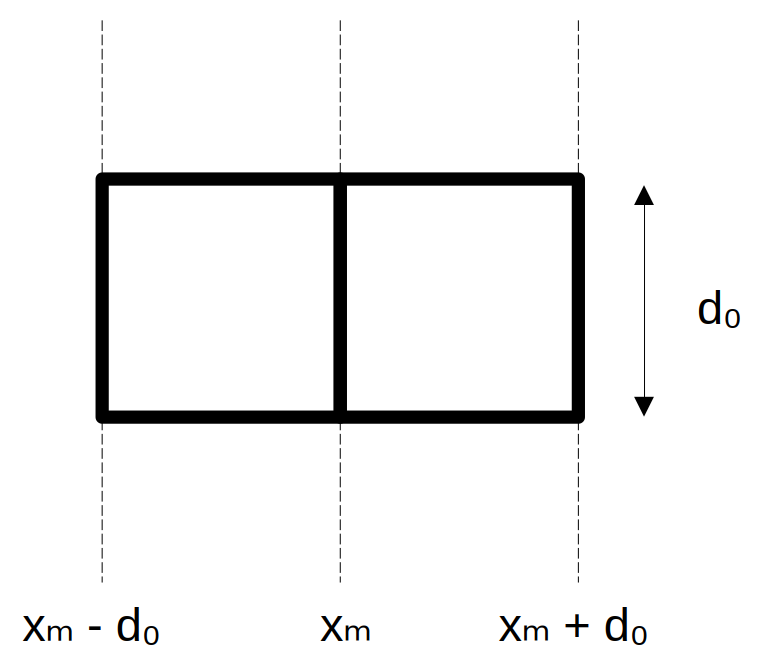
\includegraphics[width=\linewidth]{lecon/13-D&R/7_points.png}
\end{minipage}
\qquad
\begin{minipage}{0.5\linewidth}
	On a au plus 8 éléments dans ce rectangle, car dans chaque domaine, les points sont au moins à distance $d_0$. On a donc au plus $4$ points par carré, d'où le résultat en mettant notre point sur le bas du rectangle.
\end{minipage}

\begin{proposition}
	On a une complexité en $O\left(n (\log n)^2\right)$
\end{proposition}




\subsection{Arbre K-dimensionnel}

\textbf{Problème :} Trouver les $k$ plus proches voisins d'un point $y \in \mathbb R^K$ parmi un ensemble de $n$ points $x_1, \dots, x_n \in \mathbb R^K$

\textbf{Solution initiale :} Stocker nos $k$ valeurs en cours dans une file de priorité et parcourir les n points, en mettant à jour la file de priorité. $\to O(n \log k)$

\begin{algo}[Solution D\&R]
	Faire un pré traitement où l'on stockera nos valeurs dans un arbre binaire de recherche, où l'on partitionnera récursivement les données alternativement sur chaque dimension. La recherche se fait alors en ne cherchant que d'un côté si le deuxième n'est pas nécessaire.
\end{algo}

\textbf{Développement :} Présentation de la structure d'arbre K-dimensionnel

\begin{proposition}[Complexité]\enspace
	\begin{itemize}
		\item prétraitement : $O(n \log(n))$
		\item Recherche des $k$ plus proches voisins : $O(\log n \times k)$ en moyenne, $O(N \times K)$ dans le pire des cas
	\end{itemize}
\end{proposition}


\begin{rem}
	On y perd pour une seule recherche, mais si on cherche les $k$-plus proches voisins de $N$ points, on obtient du $O(n \log n + N \times k \times \log n)$ au lieu de $O(N \times n \times \log k)$.
\end{rem}

\begin{com}
	Si il reste beaucoup de places ou si on veut enlever un exemple au dessus (comme le tri rapide faisant doublons avec le tri fusion, même si il est très classique), on peut rajouter une section supplémentaire ici, et parler de l'additionneur à retenue anticipée par méthode D\&R du développement *à compléter*
\end{com}